\documentclass[aspectratio=169, 10pt]{beamer}
% ==============================================================================
% Quantum Computing 12-Hour Course: Common LaTeX Beamer Preamble
% ==============================================================================
\usepackage{amsmath, amssymb, amsfonts, mathtools}
\usepackage{booktabs}
\usepackage{kotex}
\usepackage{tikz}
\usetikzlibrary{arrows.meta, positioning, shapes.geometric, calc}

% Syntax highlighting & listings
\usepackage{listings}
\usepackage{xcolor}

\definecolor{qcDarkBlue}{RGB}{20, 35, 60}
\definecolor{qcAccentBlue}{RGB}{0, 114, 206}
\definecolor{qcTeal}{RGB}{0, 168, 150}
\definecolor{qcLightGray}{RGB}{246, 248, 251}
\definecolor{qcCodeBg}{RGB}{242, 244, 247}
\definecolor{qcKeyword}{RGB}{140, 30, 120}
\definecolor{qcString}{RGB}{30, 120, 50}
\definecolor{qcComment}{RGB}{110, 110, 120}

\lstset{
    backgroundcolor=\color{qcCodeBg},
    basicstyle=\ttfamily\scriptsize,
    keywordstyle=\color{qcKeyword}\bfseries,
    stringstyle=\color{qcString},
    commentstyle=\color{qcComment}\itshape,
    breaklines=true,
    showstringspaces=false,
    tabsize=4,
    frame=single,
    rulecolor=\color{qcAccentBlue!30},
    numbers=left,
    numberstyle=\tiny\color{qcComment},
    numbersep=6pt,
    xleftmargin=10pt,
    xrightmargin=5pt
}

% Beamer Theme Settings
\usefonttheme[onlymath]{serif}
\setbeamertemplate{navigation symbols}{}
\setbeamercolor{palette primary}{bg=qcDarkBlue, fg=white}
\setbeamercolor{palette secondary}{bg=qcAccentBlue, fg=white}
\setbeamercolor{palette tertiary}{bg=qcTeal, fg=white}
\setbeamercolor{structure}{fg=qcAccentBlue}
\setbeamercolor{titlelike}{parent=palette primary}
\setbeamercolor{frametitle}{bg=qcDarkBlue, fg=white}

% Blocks (Tight padding to prevent vertical overflow)
\usepackage{tcolorbox}
\tcbuselibrary{skins, breakable}

\newtcolorbox{qcblock}[1]{
    colback=qcLightGray,
    colframe=qcAccentBlue,
    fonttitle=\bfseries\footnotesize\color{white},
    coltitle=white,
    title={#1},
    arc=1.5mm,
    boxrule=0.8pt,
    left=5pt, right=5pt, top=3pt, bottom=3pt,
    boxsep=1pt,
    before=\vspace{2pt},
    after=\vspace{2pt}
}

\newtcolorbox{qcalert}[1]{
    colback=red!5,
    colframe=red!75!black,
    fonttitle=\bfseries\footnotesize\color{white},
    title={#1},
    arc=1.5mm,
    boxrule=0.8pt,
    left=5pt, right=5pt, top=3pt, bottom=3pt,
    boxsep=1pt,
    before=\vspace{2pt},
    after=\vspace{2pt}
}

\newtcolorbox{qctip}[1]{
    colback=green!5,
    colframe=qcTeal,
    fonttitle=\bfseries\footnotesize\color{white},
    title={#1},
    arc=1.5mm,
    boxrule=0.8pt,
    left=5pt, right=5pt, top=3pt, bottom=3pt,
    boxsep=1pt,
    before=\vspace{2pt},
    after=\vspace{2pt}
}

% Quantum Dirac Notation Macros
\newcommand{\ket}[1]{|#1\rangle}
\newcommand{\bra}[1]{\langle#1|}
\newcommand{\braket}[2]{\langle#1|#2\rangle}
\newcommand{\ketbra}[2]{|#1\rangle\langle#2|}
\newcommand{\normsq}[1]{|#1|^2}


\title[양자컴퓨팅 부트캠프 1일차]{양자컴퓨팅 이론\&실습 4주 부트캠프}
\subtitle{1일차: 단일 큐비트와 상태벡터 (NumPy 기초)}
\author{강사: 서상협 ((주)큐렌스)}
\date{2026. 11. 11 (수)}

\begin{document}

\frame{\titlepage}

% -----------------------------------------------------------------------------
\begin{frame}{수업 전 실습 준비}{1일차 교재 및 실습 파일 다운로드}
    \begin{columns}[c]
        \begin{column}{0.38\textwidth}
            \begin{center}
                
\includegraphics[width=0.62\linewidth]{qr_day1.png}\\[0.2cm]
                \textbf{\footnotesize \url{https://github.com/saibie/}}\\
                \textbf{\scriptsize quantum-computing-bootcamp-2026-day1}\\[0.15cm]
                \tiny $\uparrow$ 카메라로 QR 코드를 스캔하거나 웹 브라우저로 접속
            \end{center}
        \end{column}
        \begin{column}{0.60\textwidth}
            \begin{qcblock}{실습 교재 및 환경 다운로드 (가장 추천)}
                \begin{enumerate}
                    \item 위 저장소 우측 상단의 초록색 \textbf{[Code]} 버튼 클릭
                    \item \textbf{[Download ZIP]} 클릭하여 실습 파일 다운로드
                    \item 다운로드 완료 후 편한 폴더에 \textbf{압축 해제} (※ 압축 풀기 필수!)
                \end{enumerate}
                \vspace{0.05cm}
                {\scriptsize ※ Git 사용자는 저장소 페이지(README)에서 clone 명령어 복사 가능}
            \end{qcblock}
            \vspace{0.15cm}
            \begin{qcalert}{수업 진행 안내}
                \textbf{1부 이론(75분)} 진행 동안 다운로드 및 압축 해제까지만 진행\\
                (원클릭 환경 실행은 2부 실습 시간에 함께 진행)
            \end{qcalert}
        \end{column}
    \end{columns}
\end{frame}

% -----------------------------------------------------------------------------
\begin{frame}{강사 소개}{수치선형대수학 전공 및 연구 배경}
    \begin{columns}[c]
        \begin{column}{0.28\textwidth}
            \begin{center}
                \fboxsep=0pt\fboxrule=0.6pt\fcolorbox{gray!50}{white}{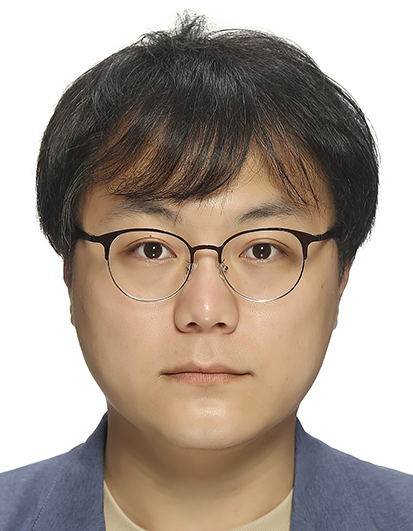
\includegraphics[width=0.68\linewidth]{photo.jpg}}\\[0.25cm]
                \textbf{\Large 서상협} \ {\small 이학박사}\\[0.15cm]
                {\scriptsize \textbf{qRens} / Quantum Computing}\\[0.2cm]
                {\tiny \textbf{Email}: \href{mailto:saibie1677@qrens.com}{\ttfamily saibie1677@qrens.com}}
            \end{center}
        \end{column}
        \begin{column}{0.70\textwidth}
            \begin{qcblock}{학력 및 연구 경력 (Education \& Career)}
                \begin{itemize}\setlength{\itemsep}{1pt}
                    \item \textbf{부산대학교 수학과 이학박사} (수치선형대수학 전공, 2019)\\
                    {\footnotesize 비선형 행렬방정식 가속 수치해법 및 행렬 해석 연구}
                    \item \textbf{(주)큐렌스 (qRens) 연구원} (2026.03 -- 현재)\\
                    {\footnotesize 양자컴퓨팅 소프트웨어 및 양자 알고리즘 연구}
                    \item \textbf{前 국가수리과학연구소 (NIMS) 박사후연구원} (2019 -- 2022)\\
                    {\footnotesize 산업수학 문제해결 연구 (Industrial Mathematics)}
                \end{itemize}
            \end{qcblock}
            \vspace{0.12cm}
            \begin{qctip}{전문 연구 분야 (Research Expertise)}
                \begin{itemize}\setlength{\itemsep}{1pt}
                    \item \textbf{수치선형대수학 (Numerical Linear Algebra)}:\\
                    행렬 다항식 고유값 문제, 비선형 행렬방정식 가속 수치 알고리즘
                \end{itemize}
            \end{qctip}
        \end{column}
    \end{columns}
\end{frame}

% -----------------------------------------------------------------------------
\begin{frame}{1일차 강의의 출발점}
    \begin{center}
        \LARGE \textbf{``선형대수학의 벡터와 행렬은\\어떻게 새로운 계산 장치의 정보 단위(큐비트)가 되는가?''}
    \end{center}
    \vspace{0.4cm}
    \begin{qcblock}{1일차 학습의 관점: 선형대수학으로 이해하는 정보의 표현과 연산}
        \begin{itemize}
            \item 고전 컴퓨터가 전압 스위치(0과 1)로 정보를 다루었다면, 양자컴퓨터는 \textbf{복소수 벡터 공간의 상태벡터}로 정보를 다룸.
            \item 난해한 양자역학 물리학 지식을 배경으로 하지 않고도, \textbf{선형대수학으로 정립된 엄밀한 연산 규칙과 하드웨어 제어 원리}를 학습함.
            \item \textbf{개념 탐구 $\to$ 핵심 규칙 정립 $\to$ 기하학적 시각화 $\to$ 손계산 검증 $\to$ NumPy 코드 시뮬레이션}의 흐름으로 원리를 확인함.
        \end{itemize}
    \end{qcblock}
\end{frame}

% -----------------------------------------------------------------------------
\begin{frame}{1일차 세부 운영안}
    \begin{center}
    \resizebox{0.95\textwidth}{!}{%
    \begin{tabular}{clcp{7.5cm}}
    \toprule
    \textbf{구간} & \textbf{주제} & \textbf{시간} & \textbf{학습자 인지 궤적 및 활동} \\
    \midrule
    \textbf{1부} & \textbf{이론} & 75분 & 비트 $\to$ 큐비트 $\to$ 상태벡터 $\to$ 사영 측정(Born) $\to$ 유니터리 게이트 $\to$ 위상(상대 위상과 간섭) $\to$ \textbf{[손계산 워크시트]} \\
    \midrule
    \textbf{휴식} & \textbf{휴식 및 실습 환경 점검} & 20분 & 재충전, 질문 및 Python/NumPy 실습 환경(\texttt{uv}, Jupyter) 확인 \\
    \midrule
    \textbf{2부} & \textbf{NumPy 인터랙티브 실습} & 75분 & \texttt{day1\_numpy\_statevector.ipynb} 실행: 게이트 유니터리성 전수 검증, 위상 간섭 시뮬레이션, 1024 Shots 통계 수렴 관찰, 1일차 총정리 \\
    \bottomrule
    \end{tabular}%
    }
    \end{center}
\end{frame}

% -----------------------------------------------------------------------------
\begin{frame}{정보의 물리적 실체}{고전 비트(Bit)는 어떻게 구현되는가?}
    \begin{qcblock}{정보는 물리계의 상태(Physical State)에 부호화됨}
        \begin{itemize}
            \item 컴퓨터의 정보는 추상적 기호에 머무르지 않고, 반드시 실제 물리 장치에 기록됨.
            \item 고전 컴퓨터의 비트(Bit): \\ 트랜지스터 전압 ($0\,\mathrm{V} \implies 0, \; 5\,\mathrm{V} \implies 1$), 플래시 메모리 전하, 하드디스크의 자화 방향.
        \end{itemize}
    \end{qcblock}
    \vspace{0.2cm}
    \begin{qcalert}{고전 비트의 물리적 제약}
        \begin{itemize}
            \item 거시적 물리 스위치는 서로 배타적인 \textbf{2가지 확정된 상태 $\{0, 1\}$ 중 오직 하나}\\ 만을 취함.
            \item 스위치가 켜져 있거나 꺼져 있는 중간 상태는 노이즈로 간주되어 회로적으로 차단
            \item 따라서 고전 비트 1개의 정보 용량은 언제나 이진 집합 $\{0, 1\}$의 원소 하나로 한정
        \end{itemize}
    \end{qcalert}
\end{frame}

% -----------------------------------------------------------------------------
\begin{frame}{양자 정보의 최소 단위}{큐비트(Qubit, Quantum Bit)란 무엇인가?}
    \begin{qcblock}{큐비트의 물리적 실체: 2-준위 미시 양자계 (Two-Level System)}
        큐비트(Qubit)는 \textbf{서로 명확히 구별되는 2개의 물리적 기저 상태}를 갖는 미시 양자계:
        \begin{itemize}
            \item \textbf{초전도 인공원자 (IBM, Google)}: 극저온 조셉슨 접합 회로의 기저 상태 vs 들뜬 상태
            \item \textbf{포획된 이온 (IonQ)}: 전자기장에 갇힌 이온의 전자 에너지 준위
            \item \textbf{광자 (Photon)}: 빛의 수평 편광 vs 수직 편광
        \end{itemize}
    \end{qcblock}
    \vspace{0.2cm}
    \begin{qctip}{미시 물리계와 거시 스위치의 결정적 차이}
        \begin{itemize}
            \item 거시 스위치는 0 또는 1 중 하나에만 정적으로 고정.
            \item 반면 미시 양자계는 자연계의 파동 원리에 의해 \textbf{두 물리적 상태가 연속적인 위상과 비율로 공존(중첩)} 가능.
        \end{itemize}
    \end{qctip}
\end{frame}

% -----------------------------------------------------------------------------
\begin{frame}{물리계에서 선형대수학으로}{계산 기저(Basis)와 Dirac 표기법}
    \begin{qcblock}{두 물리적 기준 상태를 선형대수학 정규직교기저로 정의}
        서로 직교하는 두 물리 상태를 구별하기 위해 2차원 표준 직교기저 부여:
        $$\text{기준 상태 0} \implies \ket{0} = \begin{pmatrix} 1 \\ 0 \end{pmatrix}, \qquad \text{기준 상태 1} \implies \ket{1} = \begin{pmatrix} 0 \\ 1 \end{pmatrix}$$
    \end{qcblock}
    \vspace{0.15cm}
    \begin{qcblock}{Dirac bra-ket 표기법: 열벡터와 켤레 전치 행벡터}
        \begin{itemize}
            \item \textbf{Ket $\ket{\psi}$}: 세로로 서 있는 \textbf{열벡터(Column Vector)} $\begin{pmatrix} \alpha \\ \beta \end{pmatrix}$
            \item \textbf{Bra $\bra{\psi}$}: 가로로 누운 \textbf{켤레 전치 행벡터} $\ket{\psi}^* = \begin{pmatrix} \overline{\alpha} & \overline{\beta} \end{pmatrix}$
            \item \textbf{내적(Inner Product)}: 행벡터와 열벡터의 단순 행렬곱
            $$\braket{\psi}{\psi} = \ket{\psi}^* \ket{\psi} = \begin{pmatrix} \overline{\alpha} & \overline{\beta} \end{pmatrix}\begin{pmatrix} \alpha \\ \beta \end{pmatrix} = |\alpha|^2 + |\beta|^2$$
        \end{itemize}
    \end{qcblock}
\end{frame}

% -----------------------------------------------------------------------------
\begin{frame}{양자컴퓨팅의 핵심 규칙 (1)}{상태는 기저벡터의 선형결합(중첩)으로 표현}
    \begin{qcblock}{규칙 1: 단일 큐비트 상태의 수학적 모델}
        2-준위 미시계의 임의의 상태는 두 정규직교기저의 \textbf{복소 선형결합(Linear Combination)}으로 표현:
        $$\ket{\psi} = \alpha\ket{0} + \beta\ket{1} = \alpha\begin{pmatrix} 1 \\ 0 \end{pmatrix} + \beta\begin{pmatrix} 0 \\ 1 \end{pmatrix} = \begin{pmatrix} \alpha \\ \beta \end{pmatrix} \in \mathbb{C}^2 \qquad (\alpha, \beta \in \mathbb{C})$$
    \end{qcblock}
    \vspace{0.2cm}
    \begin{qctip}{선형결합으로서의 중첩(Superposition)}
        \begin{itemize}
            \item ``중첩''이란 \textbf{선형대수학의 정규직교기저들을 복소수 계수로 선형결합한 상태}.
            \item 계수 $\alpha, \beta$를 \textbf{확률 진폭(Probability Amplitude)}이라 칭함.
            \item 큐비트 연산 도중 상태벡터는 두 기저 상태의 진폭 정보를 동시에 유지.
        \end{itemize}
    \end{qctip}
\end{frame}

% -----------------------------------------------------------------------------
\begin{frame}{복소수 진폭이 필요한 이유}{위상(Phase)과 간섭}
    \begin{qcblock}{왜 실수가 아니라 복소수($\mathbb{C}$)인가?}
        \begin{itemize}
            \item 양자 상태는 파동의 특성을 가지므로, 크기뿐만 아니라 \textbf{회전 각도인 위상(Phase)}을 가짐.
            \item 복소수 극형식 $z = r e^{i\phi}$로 위상 회전과 파동의 성질을 완벽히 기술 가능.
            \item 이 복소 위상이 존재하기 때문에 향후 다룰 \textbf{파동 간섭(상쇄 간섭과 보강 간섭)}의 수학적 설계가 가능.
        \end{itemize}
    \end{qcblock}
    \vspace{0.2cm}
    \begin{qcblock}{복소수 연산의 기본 약속}
        $z = a + bi$일 때, 켤레 복소수는 $\overline{z} = a - bi$, 크기의 제곱은 $|z|^2 = \overline{z}z = a^2 + b^2 \ge 0$.
    \end{qcblock}
\end{frame}

% -----------------------------------------------------------------------------
\begin{frame}{양자컴퓨팅의 핵심 규칙 (2)}{사영 측정(Measurement)과 Born 규칙}
    \begin{qcalert}{규칙 2: Born의 사영 측정 규칙}
        상태벡터 $\ket{\psi} = \alpha\ket{0} + \beta\ket{1}$를 외부 계측기로 관측할 때 발생하는 물리 현상:
        \begin{enumerate}
            \item 기저 $0$이 관측될 확률은 위쪽 계수의 크기 제곱: $P(0) = |\alpha|^2$
            \item 기저 $1$이 관측될 확률은 아래쪽 계수의 크기 제곱: $P(1) = |\beta|^2$
            \item 측정하는 순간 상태벡터는 관측된 축($\ket{0}$ 또는 $\ket{1}$)으로 \textbf{정사영 붕괴}함.
        \end{enumerate}
    \end{qcalert}
    \vspace{0.15cm}
    \begin{qcblock}{정규화 조건: 상태벡터는 2차원 복소 단위벡터임}
        모든 경우의 수에 대한 확률의 합은 반드시 $1$:
        $$P(0) + P(1) = |\alpha|^2 + |\beta|^2 = 1 \iff \|\ket{\psi}\|_2 = 1$$
        $\implies$ \textbf{``따라서 단일 큐비트 상태는 $\mathbb{C}^2$ 공간의 길이가 1인 단위벡터로 표현됨!''}
    \end{qcblock}
\end{frame}

% -----------------------------------------------------------------------------
\begin{frame}{양자 상태의 관측 특성}{내부 진폭과 통계적 샷(Shot) 샘플링}
    \begin{qcblock}{내부 복소 진폭과 계측기 출력의 관계}
        \begin{itemize}
            \item 고전 메모리의 값은 데이터 손상 없이 읽어서 화면에 그대로 출력 가능.
            \item 반면 큐비트의 \textbf{내부 복소수 진폭($\alpha, \beta$)}은 계측기로 직접 읽어낼 수 있는 물리량 아님.
            \item 1회 측정 시 계측기가 출력하는 신호는 오직 \textbf{0 또는 1 (고전 비트 하나)}뿐임.
        \end{itemize}
    \end{qcblock}
    \vspace{0.2cm}
    \begin{qctip}{통계적 샘플링(Shot Sampling)의 필수성}
        \begin{itemize}
            \item 단 한 번의 측정으로는 내부 확률 분포($|\alpha|^2, |\beta|^2$)를 알 수 없음.
            \item 동일한 양자 회로를 수백~수천 번 반복 실행(Shots)하여 얻은 \textbf{측정 빈도(Counts)}를 집계함으로써 비로소 확률 분포를 추정함.\\(이조차 $\alpha$, $\beta$를 직접적으로 추정하는 것이 아님.)
        \end{itemize}
    \end{qctip}
\end{frame}

% -----------------------------------------------------------------------------
\begin{frame}{[1부 손계산 워크시트 1] 임의의 상태벡터 정규화와 측정 확률}
    \begin{qcblock}{문제: 다음 단일 큐비트 상태벡터 분석}
        $$\ket{\psi} = \frac{1}{\sqrt{3}}\ket{0} + \sqrt{\frac{2}{3}}i\ket{1} = \begin{pmatrix} \frac{1}{\sqrt{3}} \\ \sqrt{\frac{2}{3}}i \end{pmatrix}$$
    \end{qcblock}
    \vspace{0.2cm}
    \begin{qctip}{직접 계산해볼 3가지 질문}
        \begin{enumerate}
            \item \textbf{[정규화 검증]}: 내적 $\braket{\psi}{\psi} = \ket{\psi}^* \ket{\psi}$를 계산하여 전체 확률이 $1$인지 검증
            \item \textbf{[측정 확률]}: 기저 $0$과 $1$이 측정될 확률 $P(0)$과 $P(1)$은 각각 몇 $\%$인가?
            \item \textbf{[사영 붕괴]}: 만약 계측기에서 $0$이 관측되었다면, 측정 직후 큐비트의 상태는 어떻게 변하는지 확인
        \end{enumerate}
    \end{qctip}
\end{frame}

% -----------------------------------------------------------------------------
\begin{frame}{[손계산 워크시트 1 풀이] 정규화 조건과 사영 붕괴 확인}
    \begin{qcblock}{1. 내적 계산을 통한 단위벡터 검증}
        $$\braket{\psi}{\psi} = \begin{pmatrix} \frac{1}{\sqrt{3}} & -\sqrt{\frac{2}{3}}i \end{pmatrix}\begin{pmatrix} \frac{1}{\sqrt{3}} \\ \sqrt{\frac{2}{3}}i \end{pmatrix} = \left|\frac{1}{\sqrt{3}}\right|^2 + \left|\sqrt{\frac{2}{3}}i\right|^2 = \frac{1}{3} + \frac{2}{3} = \mathbf{1}$$
    \end{qcblock}
    \vspace{0.15cm}
    \begin{qcblock}{2. Born 규칙에 따른 측정 확률}
        $$P(0) = \left|\frac{1}{\sqrt{3}}\right|^2 = \frac{1}{3} \approx \mathbf{33.3\%}, \qquad P(1) = \left|\sqrt{\frac{2}{3}}i\right|^2 = \frac{2}{3} \approx \mathbf{66.7\%}$$
    \end{qcblock}
    \vspace{0.15cm}
    \begin{qcalert}{3. 사영 붕괴: $0$ 관측 직후의 상태}
        측정 전 공존하던 복소 진폭 $\sqrt{\frac{2}{3}}i$는 완전히 소멸하고, 오직 관측된 기저 축으로 붕괴:
        $$\ket{\psi_{\mathrm{after}}} = \ket{0} = \begin{pmatrix} 1 \\ 0 \end{pmatrix} \quad (\text{다시 측정해도 항상 0 관측})$$
    \end{qcalert}
\end{frame}

% -----------------------------------------------------------------------------
\begin{frame}{고전 비트와 큐비트의 본질적 비교}
    \begin{center}
    \resizebox{0.95\textwidth}{!}{%
    \begin{tabular}{lll}
    \toprule
    \textbf{구분} & \textbf{고전 비트 (Classical Bit)} & \textbf{양자 큐비트 (Qubit)} \\
    \midrule
    \textbf{물리적 실체} & 2진 스위치 전압 레벨 & 2준위 양자계 (초전도 접합, 광자 등) \\
    \textbf{수학적 모델} & 이산 집합 $\{0, 1\}$ & 복소 2차원 내적 공간 $\mathbb{C}^2$의 단위벡터 \\
    \textbf{상태 변화} & 불리언 논리 게이트 (NOT, AND, OR) & 벡터의 길이를 보존하는 유니터리 변환 $U$ ($U^* U = I$) \\
    \textbf{결과 확인} & 언제든 값의 손상 없이 읽기 가능 & 측정 순간 확률적으로 0 또는 1로 투영 ($P=|\alpha|^2$) \\
    \bottomrule
    \end{tabular}%
    }
    \end{center}
    \vspace{0.3cm}
    \begin{qcblock}{핵심 메시지}
        큐비트는 \textbf{선형대수학의 복소 열벡터와 유니터리 행렬곱으로 제어되는 새로운 정보 단위}.
    \end{qcblock}
\end{frame}

% -----------------------------------------------------------------------------
\begin{frame}{블로흐 구 (Bloch Sphere)}{3차원으로 펼쳐지는 큐비트와 $\ket{\psi}$의 물리적 실체}
    \vspace{-0.1cm}
    \begin{columns}[c,onlytextwidth]
    \begin{column}{0.38\textwidth}
        \centering
        \begin{tikzpicture}[scale=0.95, >=Latex]
            \shade[ball color=qcAccentBlue!15, opacity=0.35] (0, 0) circle (1.25cm);
            \draw[thick, qcDarkBlue!70] (0, 0) circle (1.25cm);

            \draw[dashed, gray!60, thin] (1.25, 0) arc (0:180:1.25cm and 0.38cm);
            \draw[thick, qcAccentBlue!70] (-1.25, 0) arc (180:360:1.25cm and 0.38cm);

            \draw[dashed, gray!40, thin] (0, 1.25) arc (90:270:0.38cm and 1.25cm);
            \draw[qcAccentBlue!30, thin] (0, 1.25) arc (90:-90:0.38cm and 1.25cm);

            % 좌표축
            \draw[->, thick, qcDarkBlue] (0, -1.55) -- (0, 1.75) node[above] {\textbf{Z}};
            \draw[->, thick, qcDarkBlue] (0, 0) -- (-0.85, -0.48) node[below left] {\textbf{X}};
            \draw[dashed, gray!50] (0, 0) -- (0.85, 0.48);
            \draw[->, thick, qcDarkBlue] (0, 0) -- (1.6, 0) node[right] {\textbf{Y}};
            \draw[dashed, gray!50] (0, 0) -- (-1.25, 0);

            % 북극(0)과 남극(1) 명시
            \fill[qcDarkBlue] (0, 1.25) circle (2pt);
            \node[right, qcDarkBlue] at (0.05, 1.35) {\footnotesize \textbf{북극}: $\ket{0}$};
            \fill[qcDarkBlue] (0, -1.25) circle (2pt);
            \node[right, qcDarkBlue] at (0.05, -1.35) {\footnotesize \textbf{남극}: $\ket{1}$};

            % 상태벡터 및 정사영
            \coordinate (O) at (0, 0);
            \coordinate (P) at (0.65, 0.82);
            \coordinate (Pxy) at (0.65, -0.14);

            \draw[dashed, gray!75, thick] (P) -- (Pxy);
            \draw[dashed, gray!75, thick] (O) -- (Pxy);

            \draw[->, ultra thick, red!85!black] (O) -- (P) node[above right] {\small $\ket{\psi}$};
            \fill[red!85!black] (P) circle (1.8pt);

            \draw[->, thick, teal] (0, 0.48) arc (90:51:0.48cm);
            \node[teal] at (0.16, 0.58) {\scriptsize $\theta$};

            \draw[->, thick, purple] (-0.24, -0.13) arc (-150:-12:0.28cm and 0.14cm);
            \node[purple] at (0.05, -0.28) {\scriptsize $\phi$};
        \end{tikzpicture}
    \end{column}
    \begin{column}{0.60\textwidth}
        \begin{qcblock}{$\ket{\psi}$의 물리적 의미와 3차원 매개화}
            $$\ket{\psi} = \cos\frac{\theta}{2}\ket{0} + e^{i\phi}\sin\frac{\theta}{2}\ket{1}$$
            \begin{itemize}\setlength{\itemsep}{1pt}
                \item \textbf{물리적 실체}: 2-준위계(전자 스핀, 편광 등)가 실제로 향하는 \textbf{순수 양자 상태의 3차원 공간 방향(스핀 포인터)}.
                \item 계산에선 복소 열벡터로 다루지만, 물리적 본질은 3차원 구면 위의 고유한 방향벡터임.
            \end{itemize}
        \end{qcblock}
        \vspace{0.08cm}
        \begin{qctip}{블로흐 구의 기준축 약속: 무엇이 0이고 1인가?}
            \begin{itemize}\setlength{\itemsep}{1pt}
                \item \textbf{북극 ($\theta=0$)}: 고전 $0$에 대응하는 \textbf{$\ket{0}$}.
                \item \textbf{남극 ($\theta=\pi$)}: 고전 $1$에 대응하는 \textbf{$\ket{1}$}.
                \item \textbf{위도각 $\theta$}: $0/1$ 측정 확률 ($P(0)=\cos^2\frac{\theta}{2}$).
                \item \textbf{경도각 $\phi$}: 적도면 복소 위상 (간섭 지배).
            \end{itemize}
        \end{qctip}
    \end{column}
    \end{columns}
\end{frame}

% -----------------------------------------------------------------------------
\begin{frame}{블로흐 구 위의 6대 주요 기저 상태}{3차원 구면 극점과 직교 기저의 1:1 매핑}
    \vspace{-0.1cm}
    \begin{columns}[c,onlytextwidth]
    \begin{column}{0.38\textwidth}
        \centering
        \begin{tikzpicture}[scale=0.95, >=Latex]
            \shade[ball color=qcAccentBlue!15, opacity=0.35] (0, 0) circle (1.25cm);
            \draw[thick, qcDarkBlue!70] (0, 0) circle (1.25cm);

            % 적도면 타원
            \draw[dashed, gray!60, thin] (1.25, 0) arc (0:180:1.25cm and 0.38cm);
            \draw[thick, qcAccentBlue!70] (-1.25, 0) arc (180:360:1.25cm and 0.38cm);

            % 자오선 타원
            \draw[dashed, gray!40, thin] (0, 1.25) arc (90:270:0.38cm and 1.25cm);
            \draw[qcAccentBlue!30, thin] (0, 1.25) arc (90:-90:0.38cm and 1.25cm);

            % 좌표축
            \draw[->, thick, qcDarkBlue] (0, -1.6) -- (0, 1.8) node[above] {\textbf{Z}};
            \draw[->, thick, red!80!black] (0, 0) -- (-1.15, -0.62) node[below left] {\textbf{X}};
            \draw[dashed, red!50!gray] (0, 0) -- (0.85, 0.48);
            \draw[->, thick, teal] (0, 0) -- (1.65, 0) node[right] {\textbf{Y}};
            \draw[dashed, teal!50!gray] (0, 0) -- (-1.4, 0);

            % 6대 기저 상태 점 및 라벨
            % 1. Z축 (0과 1)
            \fill[qcDarkBlue] (0, 1.25) circle (2pt);
            \node[right, qcDarkBlue] at (0.05, 1.35) {\footnotesize \textbf{$\ket{0}$} (북)};
            \fill[qcDarkBlue] (0, -1.25) circle (2pt);
            \node[right, qcDarkBlue] at (0.05, -1.35) {\footnotesize \textbf{$\ket{1}$} (남)};

            % 2. X축 (+와 -)
            \fill[red!80!black] (-0.85, -0.48) circle (2.2pt);
            \node[above left, red!80!black] at (-0.75, -0.42) {\footnotesize \textbf{$\ket{+}$} (앞)};
            \fill[red!50!gray] (0.85, 0.48) circle (1.8pt);
            \node[above right, red!60!black] at (0.7, 0.48) {\footnotesize \textbf{$\ket{-}$} (뒤)};

            % 3. Y축 (+i와 -i)
            \fill[teal] (1.25, 0) circle (2pt);
            \node[above, teal] at (1.25, 0.08) {\footnotesize \textbf{$\ket{+i}$} (우)};
            \fill[teal!50!gray] (-1.25, 0) circle (1.8pt);
            \node[above, teal!60!black] at (-1.25, 0.08) {\footnotesize \textbf{$\ket{-i}$} (좌)};
        \end{tikzpicture}
    \end{column}
    \begin{column}{0.60\textwidth}
        \begin{qcblock}{{1. Z축 계산 기저 (북극과 남극 $\implies$ 0과 1)}}
            $$\ket{0} = \begin{pmatrix} 1 \\ 0 \end{pmatrix} \text{ (북극)}, \qquad \ket{1} = \begin{pmatrix} 0 \\ 1 \end{pmatrix} \text{ (남극)}$$
            \scriptsize $\braket{0}{1}=0$ 직교 상태가 구면에서는 $180^\circ$ 마주봄 ($\theta/2$ 효과)
        \end{qcblock}
        \vspace{0.05cm}
        \begin{qcblock}{{2. X축 균등 중첩 기저 (적도면 앞과 뒤)}}
            $$\ket{+} = \frac{\ket{0} + \ket{1}}{\sqrt{2}} \text{ (정면)}, \quad \ket{-} = \frac{\ket{0} - \ket{1}}{\sqrt{2}} \text{ (뒷면)}$$
            \scriptsize 위도 $\theta=\frac{\pi}{2}$ (적도)에 위치, $0$과 $1$의 관측 확률 $50:50$ 균등
        \end{qcblock}
        \vspace{0.05cm}
        \begin{qcblock}{{3. Y축 복소 중첩 기저 (적도면 우와 좌)}}
            $$\ket{+i} = \frac{\ket{0} + i\ket{1}}{\sqrt{2}} \text{ (우측)}, \quad \ket{-i} = \frac{\ket{0} - i\ket{1}}{\sqrt{2}} \text{ (좌측)}$$
            \scriptsize 적도면에서 위상이 $\pm 90^\circ$ 회전된 복소 중첩 상태
        \end{qcblock}
    \end{column}
    \end{columns}
\end{frame}

\begin{frame}{양자컴퓨팅의 핵심 규칙 (3)}{양자 게이트: 크기를 보존하는 유니터리 변환이자 구면 회전}
    \begin{qcblock}{규칙 3: 가역성과 유니터리(Unitary) 변환}
        닫힌 양자계의 가역적인 물리적 변화(시간 발전)를 수학적으로 기술하면 \textbf{벡터의 길이를 보존하는 유니터리 행렬} $U$가 됨.
        이에 따라 게이트 연산 후의 상태 $\ket{\psi'} = U\ket{\psi}$에서도 전체 확률의 합 $1$이 항상 완벽히 보존.
    \end{qcblock}
    \vspace{0.2cm}
    \begin{qctip}{유니터리 행렬의 핵심 성질: 물리적 가역성과 확률 보존}
        선형 변환 $U$가 벡터의 길이를 완벽히 보존하기 위한 필요충분조건:
        $$U^* U = U U^* = I \iff U^{-1} = U^*$$
        \begin{itemize}
            \item \textbf{물리적 가역성}: 모든 양자 게이트는 역행렬이 존재하여 물리적 상태 변화를 언제든 완벽히 되돌릴 수 있음.
            \item \textbf{확률 보존}: 연산 도중 상태벡터의 크기가 변하지 않으므로 전체 확률의 합이 $1$로 항상 유지.
        \end{itemize}
    \end{qctip}
\end{frame}

% -----------------------------------------------------------------------------
\begin{frame}{단일 큐비트 기본 게이트 (1)}{Pauli-X 게이트 (비트 반전)}
    \begin{qcblock}{Pauli-X 게이트 (양자컴퓨팅의 비트 반전 게이트)}
        $$X = \begin{pmatrix} 0 & 1 \\ 1 & 0 \end{pmatrix}$$
        \begin{itemize}
            \item 기저 벡터에 곱해보기:
            $$X\ket{0} = \begin{pmatrix} 0 & 1 \\ 1 & 0 \end{pmatrix}\begin{pmatrix} 1 \\ 0 \end{pmatrix} = \begin{pmatrix} 0 \\ 1 \end{pmatrix} = \ket{1}$$
            $$X\ket{1} = \begin{pmatrix} 0 & 1 \\ 1 & 0 \end{pmatrix}\begin{pmatrix} 0 \\ 1 \end{pmatrix} = \begin{pmatrix} 1 \\ 0 \end{pmatrix} = \ket{0}$$
            \item \textbf{기하학적 직관}: 블로흐 구에서 \textbf{$X$축을 중심으로 공을 $180^\circ$ 회전}시켜 북극과 남극의 위치를 맞바꿈.
        \end{itemize}
    \end{qcblock}
\end{frame}

% -----------------------------------------------------------------------------
\begin{frame}{단일 큐비트 기본 게이트 (2)}{Pauli-Y 게이트 (복소 위상 반전)}
    \begin{qcblock}{Pauli-Y 게이트 (비트 및 허수 위상 반전)}
        $$Y = \begin{pmatrix} 0 & -i \\ i & 0 \end{pmatrix}$$
        \begin{itemize}
            \item 기저 벡터에 곱해보기:
            $$Y\ket{0} = \begin{pmatrix} 0 & -i \\ i & 0 \end{pmatrix}\begin{pmatrix} 1 \\ 0 \end{pmatrix} = \begin{pmatrix} 0 \\ i \end{pmatrix} = i\ket{1}$$
            $$Y\ket{1} = \begin{pmatrix} 0 & -i \\ i & 0 \end{pmatrix}\begin{pmatrix} 0 \\ 1 \end{pmatrix} = \begin{pmatrix} -i \\ 0 \end{pmatrix} = -i\ket{0}$$
            \item \textbf{기하학적 직관}: 블로흐 구에서 \textbf{$Y$축을 중심으로 공을 $180^\circ$ 회전}시킴.
        \end{itemize}
    \end{qcblock}
\end{frame}

% -----------------------------------------------------------------------------
\begin{frame}{단일 큐비트 기본 게이트 (3)}{Pauli-Z 게이트 (위상 반전)}
    \begin{qcblock}{Pauli-Z 게이트 (위상 플립)}
        $$Z = \begin{pmatrix} 1 & 0 \\ 0 & -1 \end{pmatrix}$$
        \begin{itemize}
            \item $\ket{0}$은 그대로 두고, $\ket{1}$의 부호만 마이너스로 바꿈:
            $$Z\ket{0} = \ket{0}, \qquad Z\ket{1} = -\ket{1}$$
            \item 적도면 상태에 가했을 때의 놀라운 변화:
            $$Z\ket{+} = Z\left(\frac{\ket{0}+\ket{1}}{\sqrt{2}}\right) = \frac{\ket{0}-\ket{1}}{\sqrt{2}} = \ket{-}$$
            \item \textbf{기하학적 직관}: 블로흐 구에서 \textbf{$Z$축(자전축)을 중심으로 공을 $180^\circ$ 회전}시켜 적도면의 정면($\ket{+}$)을 뒷면($\ket{-}$)으로 보냄.
        \end{itemize}
    \end{qcblock}
\end{frame}

% -----------------------------------------------------------------------------
\begin{frame}{단일 큐비트 기본 게이트 (4)}{Hadamard 게이트 ($H$)}
    \begin{qcalert}{양자컴퓨팅에서 가장 중요한 게이트: Hadamard ($H$)}
        고전 비트 상태(0 또는 1)를 반반 중첩 상태로 만드는 핵심 연산자:
        $$H = \frac{1}{\sqrt{2}}\begin{pmatrix} 1 & 1 \\ 1 & -1 \end{pmatrix}$$
    \end{qcalert}
    \vspace{0.2cm}
    \begin{qcblock}{Hadamard의 역할: 북극을 적도로 눕히기}
        \begin{itemize}
            \item 북극 $\ket{0}$에 $H$를 걸면 적도의 $\ket{+}$가 됨:
            $$H\ket{0} = \frac{1}{\sqrt{2}}\begin{pmatrix} 1 & 1 \\ 1 & -1 \end{pmatrix}\begin{pmatrix} 1 \\ 0 \end{pmatrix} = \frac{1}{\sqrt{2}}\begin{pmatrix} 1 \\ 1 \end{pmatrix} = \ket{+}$$
            \item 남극 $\ket{1}$에 $H$를 걸면 반대편 적도의 $\ket{-}$가 됨:
            $$H\ket{1} = \frac{1}{\sqrt{2}}\begin{pmatrix} 1 & 1 \\ 1 & -1 \end{pmatrix}\begin{pmatrix} 0 \\ 1 \end{pmatrix} = \frac{1}{\sqrt{2}}\begin{pmatrix} 1 \\ -1 \end{pmatrix} = \ket{-}$$
        \end{itemize}
    \end{qcblock}
\end{frame}

% -----------------------------------------------------------------------------
\begin{frame}{[손계산 실습] Hadamard 게이트를 두 번 통과하면?}
    \begin{qcblock}{의문: 중첩을 한 번 더 통과시키면 더 섞일까?}
        적도에 누워 있는 $\ket{+}$ 상태에 $H$ 게이트를 한 번 더 곱해보면:
        $$H\ket{+} = \frac{1}{\sqrt{2}}\begin{pmatrix} 1 & 1 \\ 1 & -1 \end{pmatrix} \frac{1}{\sqrt{2}}\begin{pmatrix} 1 \\ 1 \end{pmatrix} = \frac{1}{2}\begin{pmatrix} 1 + 1 \\ 1 - 1 \end{pmatrix} = \begin{pmatrix} 1 \\ 0 \end{pmatrix} = \ket{0}$$
    \end{qcblock}
    \vspace{0.2cm}
    \begin{qctip}{Hadamard 게이트 2회 작용의 의미: 가역성의 회복}
        \begin{itemize}
            \item 중첩 상태가 더 무질서하게 섞이는 것이 아니라, \textbf{정확하게 원래의 북극 $\ket{0}$으로 복귀}!
            \item 아래쪽 성분에서 $1 - 1 = 0$이 되는 것은 양자 간섭(상쇄)의 가장 단순한 형태임.
            \item 양자 게이트 연산은 확률이 흩어지는 것이 아니라, 철저히 통제된 기하학적 회전임을 보여줌.
        \end{itemize}
    \end{qctip}
\end{frame}

% -----------------------------------------------------------------------------
\begin{frame}{단일 큐비트 기본 게이트 (5)}{위상 게이트 ($S, T$)}
    \begin{qcblock}{Phase 게이트 ($S$)와 $T$ 게이트}
        Z축을 기준으로 미세한 각도만큼 회전시키는 유니터리 연산자:
        $$S = \begin{pmatrix} 1 & 0 \\ 0 & i \end{pmatrix} = \begin{pmatrix} 1 & 0 \\ 0 & e^{i\pi/2} \end{pmatrix}, \qquad T = \begin{pmatrix} 1 & 0 \\ 0 & e^{i\pi/4} \end{pmatrix}$$
    \end{qcblock}
    \vspace{0.2cm}
    \begin{qctip}{게이트 간의 대수적 포함 관계}
        \begin{itemize}
            \item $S$는 $Z$의 제곱근 ($S^2 = Z$): 블로흐 구 $Z$축을 기준으로 \textbf{$90^\circ$ 회전}
            \item $T$는 $S$의 제곱근 ($T^2 = S, \; T^4 = Z$): 블로흐 구 $Z$축을 기준으로 \textbf{$45^\circ$ 회전}
            \item 양자 알고리즘에서 정밀한 각도를 제어하기 위해 반드시 필요한 위상 게이트임.
        \end{itemize}
    \end{qctip}
\end{frame}

% -----------------------------------------------------------------------------
\begin{frame}{[1부 핵심 원리] 위상(Phase)과 양자 간섭의 원천}
    \begin{qcblock}{상태벡터에서 위상차($e^{i\phi}$)가 갖는 의미}
        단일 큐비트의 일반적인 중첩 상태는 다음과 같이 표현됨:
        $$\ket{\psi} = \alpha\ket{0} + e^{i\phi}\beta\ket{1} \quad (\alpha, \beta \ge 0)$$
        여기서 $e^{i\phi}$는 $\ket{0}$과 $\ket{1}$ 사이의 \textbf{상대적 위상차(Relative Phase)}를 나타냄.
    \end{qcblock}
    \vspace{0.15cm}
    \begin{qctip}{위상은 계산 기저 측정만으로는 보이지 않지만, 간섭을 결정함}
        \begin{itemize}
            \item 계산 기저($Z$축)로만 측정하면 $|e^{i\phi}\beta|^2 = |\beta|^2$이므로 위상 각도 $\phi$는 확률에 직접 드러나지 않음.
            \item 그러나 게이트(예: $H$)를 적용하는 순간, \textbf{위상 각도에 따라 진폭이 더해지거나(보강) 빼지는(상쇄) 양자 간섭}이 일어남!
            \item 즉, 양자컴퓨팅에서 알고리즘의 성패는 바로 이 \textbf{상대 위상을 정밀하게 조작하는 데} 달려 있음.
        \end{itemize}
    \end{qctip}
\end{frame}

% -----------------------------------------------------------------------------
\begin{frame}{[1부 손계산 워크시트 2] 왜 $\ket{+}$와 $\ket{-}$는 완전히 다른 상태인가?}
    \begin{qcblock}{겉보기 측정 확률이 동일한 두 상태}
        $$\ket{+} = \frac{\ket{0}+\ket{1}}{\sqrt{2}} = \frac{1}{\sqrt{2}}\begin{pmatrix} 1 \\ 1 \end{pmatrix}, \qquad \ket{-} = \frac{\ket{0}-\ket{1}}{\sqrt{2}} = \frac{1}{\sqrt{2}}\begin{pmatrix} 1 \\ -1 \end{pmatrix}$$
        \begin{itemize}
            \item $Z$축 계산 기저로 측정하면 둘 다 $P(0)=50\%, P(1)=50\%$로 겉보기 확률이 동일함.
        \end{itemize}
    \end{qcblock}
    \vspace{0.15cm}
    \begin{qctip}{Hadamard를 통과시키는 순간 발생하는 기적}
        $$H\ket{+} = H\left(\frac{\ket{0}+\ket{1}}{\sqrt{2}}\right) = \mathbf{\ket{0}} \implies \mathbf{100\%\text{ 확률로 0 관측!}}$$
        $$H\ket{-} = H\left(\frac{\ket{0}-\ket{1}}{\sqrt{2}}\right) = \mathbf{\ket{1}} \implies \mathbf{100\%\text{ 확률로 1 관측!}}$$
        $\implies$ \textbf{"상대 위상(부호)의 차이는 Hadamard 변환을 거쳐 100\% 확정된 비트 차이로 판별됨!"}
    \end{qctip}
\end{frame}

% -----------------------------------------------------------------------------
\begin{frame}{1부 마무리 및 중간 휴식 안내 (20분)}
    \begin{qcblock}{1부 핵심 달성도 체크}
        \begin{itemize}
            \item $\checkmark$ 큐비트의 물리적 실체(2-준위계)와 선형대수학 단위벡터 매핑
            \item $\checkmark$ Born 규칙에 따른 사영 붕괴 확률 계산 및 단위벡터 정규화 검증
            \item $\checkmark$ 유니터리 연산자($U^* U = I$)와 기본 게이트($X, Y, Z, H, S, T$)
            \item $\checkmark$ 상대 위상($\pm$)의 차이와 Hadamard 간섭($H\ket{+}=\ket{0}, H\ket{-}=\ket{1}$)
        \end{itemize}
    \end{qcblock}
    \vspace{0.25cm}
    \begin{qctip}{20분간 휴식 및 실습 환경 준비 안내}
        \begin{itemize}
            \item 휴식 후 2부에서는 \textbf{NumPy를 이용한 주피터 인터랙티브 실습(75분)} 진행
            \item 다운로드받은 실습 폴더를 열고 다음 슬라이드의 \textbf{[원클릭 실행 안내]} 확인
        \end{itemize}
    \end{qctip}
\end{frame}

% -----------------------------------------------------------------------------
\begin{frame}{2부 실습 시작}{원클릭 실행 및 동작 과정 (무슨 일이 일어나는가?)}
    \begin{columns}[t]
        \begin{column}{0.485\textwidth}
            \begin{qcblock}{1단계: 원클릭 실행기 더블 클릭}
                압축 푼 폴더 안의 실행기 실행:
                \begin{itemize}
                    \item \textbf{Windows}: \texttt{\textbf{start\_windows.bat}} 더블 클릭
                    \item \textbf{macOS / Linux}: 터미널에서 \texttt{\textbf{./start\_mac.sh}}
                \end{itemize}
                \vspace{0.02cm}
                {\tiny ※ Windows 보안 경고 시: \textbf{[추가 정보] $\to$ [실행]} 클릭}
            \end{qcblock}
            \vspace{0.04cm}
            \begin{qcalert}{2단계: 검은색 터미널 창 (※ 절대 닫지 말 것)}
                \begin{itemize}
                    \item 검은색 명령 프롬프트(CMD) 창 실행은 \textbf{정상}.
                    \item \texttt{uv}가 Python 3.12와 NumPy 환경 자동 구성
                    \item \textbf{주의}: 실습 중 창을 닫으면 주피터 서버가 종료됨!
                \end{itemize}
            \end{qcalert}
        \end{column}
        \begin{column}{0.485\textwidth}
            \begin{qcblock}{3단계: 웹 브라우저 자동 실행 및 노트북 열기}
                \begin{itemize}
                    \item 동기화 완료 후 브라우저에 \textbf{Jupyter Lab} 자동 실행됨.
                    \item 좌측에서 \texttt{\textbf{day1\_numpy\_statevector.ipynb}}를 더블 클릭하여 실습 시작!
                \end{itemize}
            \end{qcblock}
            \vspace{0.04cm}
            \begin{qctip}{문제 해결 (FAQ \& 비상 대안)}
                \begin{itemize}
                    \item \textbf{브라우저 미작동 시}: \texttt{\textbf{http://localhost:8888}} 직접 접속
                    \item \textbf{실행 오류 발생 시}: 강사/조교에게 즉시 문의
                \end{itemize}
            \end{qctip}
        \end{column}
    \end{columns}
\end{frame}

% -----------------------------------------------------------------------------
\begin{frame}{2부 시작}{Jupyter Notebook 실습 개요}
    \begin{qcblock}{실습 교재: hands\_on/day1\_numpy\_statevector.ipynb}
        외부 양자 라이브러리 없이, \textbf{순수 Python과 NumPy}만으로 양자 연산자 직접 구축:
    \end{qcblock}
    \vspace{0.2cm}
    \begin{qctip}{2부 75분 실습의 5대 Lab 구성}
        \begin{enumerate}
            \item \textbf{[Lab 1]} $2 \times 1$ 복소 배열 기저 정의 및 6대 게이트 유니터리성($U^* U = I$) 전수 검증
            \item \textbf{[Lab 2]} 게이트 행렬곱 작용과 $H^2 = I$ 가역성 복원 시뮬레이션
            \item \textbf{[Lab 3]} 상대 위상에 따른 Hadamard 양자 간섭 효과 시뮬레이션
            \item \textbf{[Lab 4]} 난수 기반 1024회 샷(Shots) 샘플링 및 측정 카운트 집계
            \item \textbf{[Lab 5]} 샷 수(10 vs 100 vs 1000 vs 8192)에 따른 대수의 법칙($1/\sqrt{M}$) 수렴 분석
        \end{enumerate}
    \end{qctip}
\end{frame}

% -----------------------------------------------------------------------------
\begin{frame}[fragile]{[Lab 1] NumPy로 정의하는 기저벡터와 유니터리 게이트}
    기저벡터와 게이트를 2차원 복소 배열로 선언하고 유니터리성 검증:
    \vspace{0.2cm}
\begin{lstlisting}[language=Python]
import numpy as np

# 1. 2차원 복소 열벡터 기저
ket0 = np.array([[1.0 + 0.0j], [0.0 + 0.0j]])  # |0>
ket1 = np.array([[0.0 + 0.0j], [1.0 + 0.0j]])  # |1>

# 2. Hadamard 게이트 행렬
H = (1.0 / np.sqrt(2.0)) * np.array([[1,  1],
                                     [1, -1]], dtype=complex)

# 3. 유니터리성 검증 함수 (U* U == I)
def check_unitary(U: np.ndarray) -> bool:
    U_dagger = U.conj().T  # Conjugate Transpose (U*)
    identity = np.eye(U.shape[0], dtype=complex)
    return np.allclose(U_dagger @ U, identity)

assert check_unitary(H), "Hadamard 게이트는 유니터리 행렬이어야 함!"
print("Hadamard 게이트 유니터리성 검증 통과!")
\end{lstlisting}
\end{frame}

% -----------------------------------------------------------------------------
\begin{frame}[fragile]{[Lab 2] 파이썬 코드로 확인하는 상태벡터와 게이트}
    손으로 계산했던 $H$ 게이트 연산과 $H^2 = I$ 가역 복원을 코드로 확인:
    \vspace{0.2cm}
\begin{lstlisting}[language=Python]
# 1. H 게이트 작용: |0> -> |+>
plus = H @ ket0
print("H|0> (|+> 상태벡터) =\n", plus)
# 출력: [[0.7071+0.j], [0.7071+0.j]]

# 2. H 게이트 재작용: H|+> -> |0> 복귀 검증
recovered_0 = H @ plus
assert np.allclose(recovered_0, ket0), "H를 두 번 통과하면 |0>으로 복귀해야 함!"

# 3. |1>에 H 게이트 작용: |1> -> |->
minus = H @ ket1
print("H|1> (|-> 상태벡터) =\n", minus)
# 출력: [[0.7071+0.j], [-0.7071+0.j]]
assert np.allclose(H @ minus, ket1), "H|->에 H를 곱하면 |1>로 복귀!"
print("가역성 복원 검증 완료!")
\end{lstlisting}
\end{frame}

% -----------------------------------------------------------------------------
\begin{frame}[fragile]{[Lab 3] 상대 위상과 양자 간섭의 NumPy 검증}
    겉보기 확률이 같은 $\ket{+}$와 $\ket{-}$가 간섭을 통해 어떻게 갈라지는지 확인:
    \vspace{0.2cm}
\begin{lstlisting}[language=Python]
# 1. 상대 위상이 0인 |+>와 pi인 |-> 상태 정의
plus  = (1 / np.sqrt(2)) * np.array([[1], [ 1]])  # (|0> + |1>) / sqrt(2)
minus = (1 / np.sqrt(2)) * np.array([[1], [-1]])  # (|0> - |1>) / sqrt(2)

# 2. 단순 Z-기저 측정 확률 비교 (둘 다 50% vs 50%로 동일)
prob_plus = np.abs(plus) ** 2
prob_minus = np.abs(minus) ** 2
assert np.allclose(prob_plus, prob_minus), "겉보기 측정 확률은 둘 다 50:50!"

# 3. Hadamard 게이트 통과: 상대 위상이 보강/상쇄 간섭을 일으킴
result_plus  = H @ plus   # 보강 간섭 -> |0> (100%)
result_minus = H @ minus  # 상쇄 간섭 -> |1> (100%)

assert np.allclose(result_plus, ket0), "|+>에 H를 걸면 보강 간섭으로 |0>!"
assert np.allclose(result_minus, ket1), "|->에 H를 걸면 상쇄 간섭으로 |1>!"
print("상대 위상에 따른 양자 간섭 검증 완료: H|+>=|0>, H|->=|1>")
\end{lstlisting}
\end{frame}

% -----------------------------------------------------------------------------
\begin{frame}[fragile]{[Lab 4] 1024번 측정(Shots) 시뮬레이션}
    이론적 확률 $50\%$가 실제 반복 측정(Shots)에서 어떻게 나타나는지 확인:
    \vspace{0.2cm}
\begin{lstlisting}[language=Python]
# |+> 상태에서 0과 1이 관측될 이론 확률 계산
prob_0 = float(np.abs(plus[0, 0]) ** 2)  # |0.7071|^2 = 0.5
prob_1 = float(np.abs(plus[1, 0]) ** 2)  # |0.7071|^2 = 0.5

# 1024번의 측정(Shot) 샘플링 시뮬레이션
np.random.seed(42)
shots = 1024
outcomes = np.random.choice([0, 1], size=shots, p=[prob_0, prob_1])

count_0 = int(np.sum(outcomes == 0))
count_1 = int(np.sum(outcomes == 1))
print(f"1024회 측정 결과: 0이 {count_0}회 ({count_0/shots*100:.1f}%), 1이 {count_1}회 ({count_1/shots*100:.1f}%)")
# 출력: 0이 515회 (50.3%), 1이 509회 (49.7%)
\end{lstlisting}
\end{frame}

% -----------------------------------------------------------------------------
\begin{frame}[fragile]{[Lab 5] 샷(Shots) 수에 따른 통계 수렴과 대수의 법칙}
    샷 수에 따라 관측 오차가 어떻게 감소하는지 실험:
    \vspace{0.2cm}
\begin{lstlisting}[language=Python]
shot_list = [10, 100, 1000, 8192]
print(f"{'Shots':>8} | {'Count 0':>8} | {'Freq 0 (%)':>10} | {'오차 (%)':>8}")
print("-" * 44)
for s in shot_list:
    draws = np.random.choice([0, 1], size=s, p=[0.5, 0.5])
    c0 = np.sum(draws == 0)
    freq0 = c0 / s * 100
    err = abs(freq0 - 50.0)
    print(f"{s:>8} | {c0:>8} | {freq0:>9.2f}% | {err:>7.2f}%")
# 샷 수가 증가할수록 오차는 1/sqrt(Shots)에 비례하여 0으로 급격히 수렴!
\end{lstlisting}
\end{frame}

% -----------------------------------------------------------------------------
\begin{frame}{[2부 도전 과제] 1-큐비트 회로 상태 추적 챌린지}
    \begin{qcblock}{도전 문제: 다음 게이트 연쇄의 최종 상태벡터 예측}
        초기 상태 $\ket{0}$에 4개의 게이트를 순서대로 적용:
        $$\ket{\psi_{\mathrm{final}}} = H \cdot Z \cdot H \cdot X \ket{0}$$
    \end{qcblock}
    \vspace{0.2cm}
    \begin{qctip}{힌트 및 단계별 손계산}
        \begin{enumerate}
            \item $X\ket{0} = \ket{1}$
            \item $H\ket{1} = \ket{-} = \frac{\ket{0}-\ket{1}}{\sqrt{2}}$
            \item $Z\ket{-} = \ket{+} = \frac{\ket{0}+\ket{1}}{\sqrt{2}}$
            \item $H\ket{+} = \mathbf{\ket{0}} = \begin{pmatrix} 1 \\ 0 \end{pmatrix}$
        \end{enumerate}
        $\implies$ \textbf{수학적 항등식}: $H Z H = X$이므로, $H Z H X = X \cdot X = I$가 되어 원래 $\ket{0}$으로 복귀!
    \end{qctip}
\end{frame}

% -----------------------------------------------------------------------------
\begin{frame}{1일차 총정리}{단일 큐비트의 수학적 모델}
    \begin{qcblock}{오늘 정리한 3대 선형대수학적 원리}
        \begin{enumerate}
            \item \textbf{상태의 본질: 2차원 복소 단위벡터}:
            단일 큐비트의 물리적 상태는 $\mathbb{C}^2$ 상의 단위벡터 $\begin{pmatrix} \alpha \\ \beta \end{pmatrix}$로 엄밀히 표현됨.
            \item \textbf{게이트의 본질: 유니터리 변환 행렬}:
            $X, Y, Z, H, S, T$ 등 모든 양자 게이트는 벡터의 크기를 보존하는 유니터리 행렬($U^* U = I$)임.
            \item \textbf{측정의 본질: Born 규칙과 사영 붕괴}:
            중첩 상태라도 측정 시 기저 $\ket{0}, \ket{1}$ 중 하나로 투영 붕괴($P(x)=|\braket{x}{\psi}|^2$)하므로, 통계적 분포를 파악하기 위해서는 반복 측정(Shot sampling)이 요구됨.
        \end{enumerate}
    \end{qcblock}
    \vspace{0.2cm}
    \begin{qctip}{2일차 예고: 다중 큐비트와 상태공간 확장}
        큐비트가 결합하면 상태공간의 차원은 왜 지수적으로 팽창($2^n$)하며, 독립된 상태로 분리할 수 없는 '얽힘'은 어떻게 만들어지는가?
    \end{qctip}
\end{frame}

\end{document}
